\usetikzlibrary{arrows}
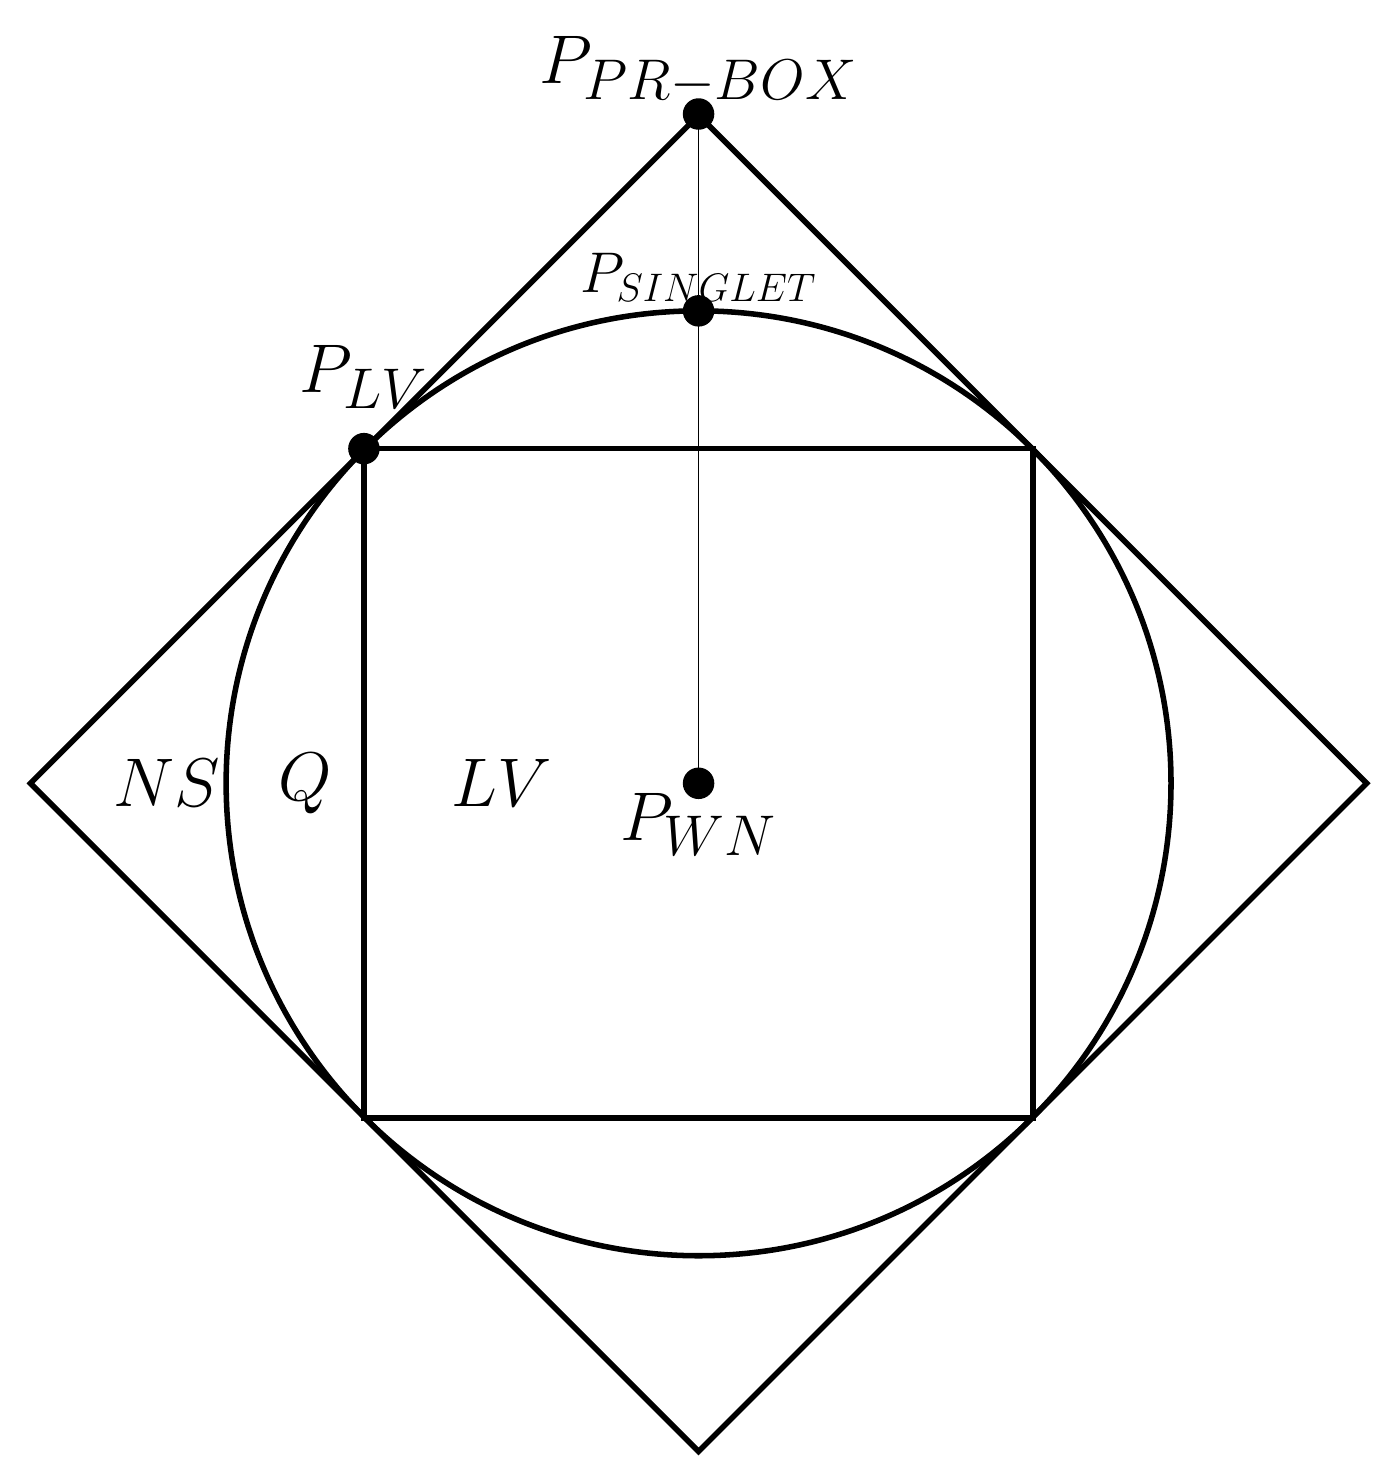
\begin{tikzpicture}

\draw[line width=2pt,rotate around={45:(0,0)}]  (-6,6) {} rectangle (6,-6);

\draw[line width=2pt]  (0,0) node (a) {} ellipse (6 and 6);
\draw[line width=2pt]  (-4.25,4.25)  node (b) {} rectangle (4.25,-4.25) ;
\fill[black] (a) circle (0.2cm);
\fill[black] (b) circle (0.2cm);
\fill[black] (0,8.5) node (c) {} circle (0.2cm);
\fill[black] (0,6) node (d) {} circle (0.2cm);

\node[below] at (a) {\Huge \color{black} $P_{WN}$};
\node[above=11] at (b) {\Huge \color{black} $P_{LV}$};
\node[above] at (c) {\Huge \color{black} $P_{PR-BOX}$};
\node[above] at (d) {\huge \color{black} $P_{SINGLET}$};
\node at (-2.5,0) {\Huge \bf \color{black} $LV$};
\node at (-5,0) {\Huge \bf \color{black} $Q$};
\node at (-6.75,0) {\Huge \bf \color{black} $NS$};

\draw  (a) edge (c);
\end{tikzpicture}